% Autor: Leonhard Segger, Alexander Neuwirth
% Datum: 2017-10-30
\documentclass[
	% Papierformat
	a4paper,
	% Schriftgröße (beliebige Größen mit „fontsize=Xpt“)
	12pt,
	% Schreibt die Papiergröße korrekt ins Ausgabedokument
	pagesize,
	% Sprache für z.B. Babel
	ngerman
]{scrartcl}

% Achtung: Die Reihenfolge der Pakete kann (leider) wichtig sein!
% Insbesondere sollten (so wie hier) babel, fontenc und inputenc (in dieser
% Reihenfolge) als Erstes und hyperref und cleveref (Reihenfolge auch hier
% beachten) als Letztes geladen werden!

% Silbentrennung etc.; Sprache wird durch Option bei \documentclass festgelegt
\usepackage{babel}
% Verwendung der Zeichentabelle T1 (Sonderzeichen etc.)
\usepackage[T1]{fontenc}
% Legt die Zeichenkodierung der Eingabedatei fest, z.B. UTF-8
\usepackage[utf8]{inputenc}
% Schriftart
\usepackage{lmodern}
% Zusätzliche Sonderzeichen
\usepackage{textcomp}

% Mathepaket (intlimits: Grenzen über/unter Integralzeichen)
\usepackage[intlimits]{amsmath}
% Ermöglicht die Nutzung von \SI{Zahl}{Einheit} u.a.
\usepackage{siunitx}
% Zum flexiblen Einbinden von Grafiken (\includegraphics)
\usepackage{graphicx}
% Abbildungen im Fließtext
\usepackage{wrapfig}
% Abbildungen nebeneinander (subfigure, subtable)
\usepackage{subcaption}
% Funktionen für Anführungszeichen
\usepackage{csquotes}
% Zitieren, Bibliographie
\usepackage{biblatex}


% Zur Darstellung von Webadressen
\usepackage{url}
%chemische Formeln
\usepackage[version=4]{mhchem}
% siunitx: Deutsche Ausgabe, Messfehler getrennt mit ± ausgeben
\usepackage{floatrow}
\usepackage{float}
\floatsetup[table]{capposition=top}
% Verlinkt Textstellen im PDF-Dokument
\usepackage[unicode]{hyperref}
% "Schlaue" Referenzen (nach hyperref laden!)
\usepackage{cleveref}
\sisetup{
	locale=DE,
	separate-uncertainty
}
\bibliography{6Mi_E3_17-01-2018_References}

\begin{document}
	
	\begin{titlepage}
		\centering
		{\scshape\LARGE Versuchsbericht zu \par}
		\vspace{1cm}
		{\scshape\huge E3 - Elektrische Resonanz \par} 
		\vspace{2.5cm}
		{\LARGE Gruppe 6Mi \par}
		\vspace{0.5cm}
		
		{\large Alexander Neuwirth (E-Mail: a\_neuw01@wwu.de) \par}
		{\large Leonhard Segger (E-Mail: l\_segg03@uni-muenster.de) \par}
		\vfill
		
		durchgeführt am 17.01.2018\par
		betreut von\par
		{\large Wladislaw Hartmann} %TODO Ich hoffe, das ist der richtige
		
		\vfill
		
		{\large \today\par}
	\end{titlepage}
	\tableofcontents
	\newpage

	%TODO mehr TODO in Default	

	\section{Kurzfassung}
	%TODO Hypothese	und deren Ergebnis
	%TODO Ergebnisse, auch Zahlen, mindestens wenn's halbwegs Sinn ergibt
	%TODO Was wurde gemacht
	In diesem Versuch wurde das elektrische Resonanzverhalten von einem Serienresonanzkreis und einem Parallelresonanzkreis untersucht.
	Dazu wurden die entsprechenden Schwingkreise durch einem Funktiongenerator zum Schwingen angeregt.
	Mit einem Multimeter wurde die Spannung über einen \SI{10}{\Omega} Widerstand in Abhängigkeit von der Kapazität des Kondensators bestimmt, da ein Variieren der Frequenz des Stroms weniger praktikabel ist, um die Resonanz des Schwingkreises quantisieren.  %TODO effektive Stromstärke und Spannung??

	Je Resonanzkreis wurde für 3 unterschiedliche  Widerstände und ca. 20 um den Resonanzfall gehäufte Kapazitäten die Stromstärke erfasst.
	Der Innenwiderstand der jeweiligen Spulen im Schwingkreis lässt sich aus der aufgenommenen Resonanzkurve bestimmen.
	Die Hypothese, dass dieser dem direkt durch das Multimeter bestimmen Innenwiderstand entsprechen muss, wurde im folgenden überprüft.

	Des Weiteren konnte aus den bestimmten Eigenfrequenzen die Induktivität der Spulen bestimmt werden.
	Für die dicke Spule im Serienresonanzkreis ergab sich eine Induktivität von \SI{0,094 \pm 0,002}{H} und für die kleine Spule im Parallelresonanzkreis \SI{0,0669 \pm 0,0003}{H}.
	%TODO Ergebnis Innenwiderstand
	%TODO ergebniss Spule L
	%ERGEBNISSE

	%TODO aufgenommene Werte vergleichen was produziert wurde.

	\section{Methoden}
	%TODO Bilder von der Website klauen
	Als Erstes wurde eine Reihenschwingkreis aufgebaut (\cref{serieAufbau}).
	Mit dem Multimeter wurde die Spannung über den \SI{10}{\Omega} Widerstand gemessen, sodass sich daraus die Strokstärke bestimmen lässt.
	Mit dem Funktiongenerator und dem Oszilloskop wurde die Frequenz des Wechselstorms auf \SI{1}{kHz} und eine Peak-Peak-Spannung von \SI{4}{V} eingestellt.

	Für 3 Widerstände (\SI{200}{\Omega}, \SI{500}{\Omega} und \SI{0}{\Omega}) wurden die am Multimeter gemessenen Spannungen in Abhängigkeit von der eingestellten Kapazität aufgenommen .
	Diese Kapazität wurde in kleinen Schritten nahe dem Resonanzfall, also maximaler Spannung, abgetastet.
	Die im Resonanzfall angezeigte Peak-Peak-Spannung am Oszilloskop wurde ebenfalls erfasst.
	Zuletzt wurde der Widerstand der Spule mit dem Multimeter gemessen.

	Die Untersuchung des Parrallelschwingkreises erfolgte analog (\cref{parallelAufbau}), jedoch mit einer anderen Spule, anderen Widerständen (\SI{2}{k\Omega}, \SI{10}{k\Omega} und $\infty$ \SI{}{k\Omega}) und einer Peak-Peak-Spannung von \SI{10}{V}.
	Ein weiterer Unterschied der Schwingkreise ist, dass im Parallelschwingkreis im Resonanzfall eine minimaler Spannung am Multimeter auftritt.
	\begin{figure}[H]
		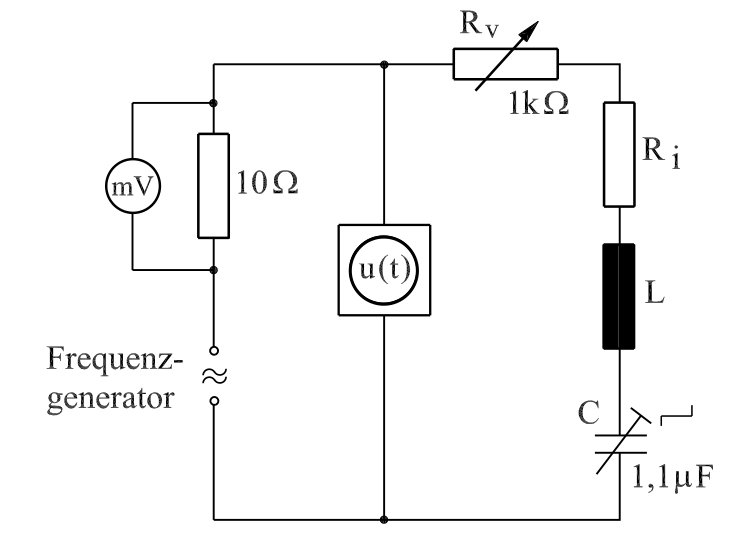
\includegraphics[width=0.5\textwidth]{serieAufbau}
		\centering
		\caption{Experimenteller Aufbau des Serienresonanzkreises.\cite{WWU}} %TODO cref/literatur von learnweb
		\label{serieAufbau}
		\centering
	\end{figure} 
		\begin{figure}[H]
		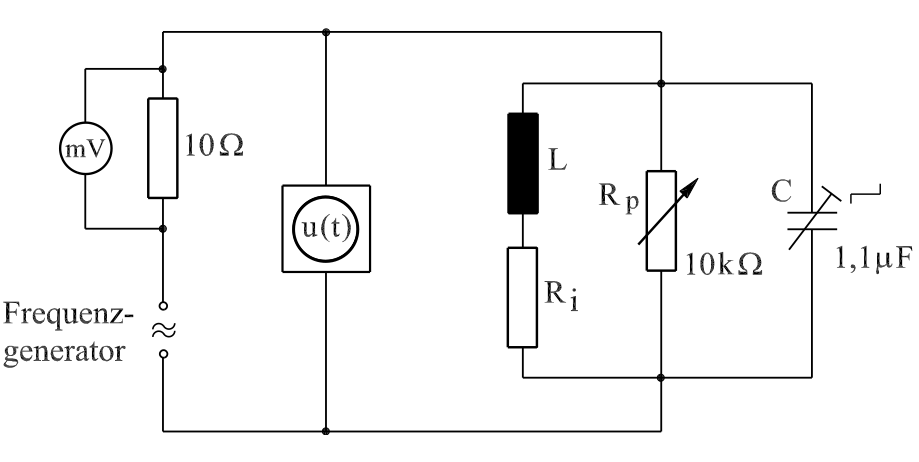
\includegraphics[width=0.5\textwidth]{parallelAufbau}
		\centering
		\caption{Experimenteller Aufbau des Parallelresonanzkreises.\cite{WWU}} %TODO KReis oder Kreises
		\label{parallelAufbau}
		\centering
	\end{figure}

	

	\section{Ergebnisse und Diskussion}
	%TODO Datenanalyse -> Überschrift?
	%TODO Unsicherheiten
	\subsection{Beobachtung}
	Für die Unsicherheit des Multimeters und des Kondensators war kein Fehler angegeben, im Folgenden wird ein Fehler von 1\% des Messwerts (mit rechteckiger WDF) angenommen. %Irgendwie sieht das %-Zeichen merkwürdig aus.
	Hierbei schwankten die Messwerte kaum.
	Zusätzlich besteht eine Unsicherheit von \SI{0,02}{mV} aufgrund der Digitalanzeige.
	Diese wurde im Fall der Widerstandsmessung vernachlässigt, da sie im Vergleich zur Unsicherheit des Mulitimeters selbst verschwindet.
	In \cref{Grundwerte} sind die Messwerte des Widerstands $R_v$ bzw. $R_p$ sowie die vom Oszilloskop angezeigte Spitze-Spitze-Spannung weit entfernt und am Resonanzfall angegeben. %Spitze-Spitze-Spannung klingt scheiße, aber w/e
	Für die Unsicherheit der Spannungsangabe des Oszilloskop wurde die Schwankung des Wertes (\SI{0,04}{\volt} mit rechteckiger WDF) zugrunde gelegt und vorausgesetzt, dass diese (weil sie relativ groß war) die Unsicherheit der Anzeige und des Messgerätes ihr gegenüber verschwinden lässt.
	\begin{table}[tb]
		\centering
		\begin{tabular}{ r | c | c | c }
			& Spannung P-P fern (\si{\volt}) & Spannung P-P nah (\si{\volt}) & Widerstand $R_v$(\si{\ohm})\\ \hline 
			S1& $4 \pm 0,012 $ & $3,6 \pm 0,012 $& $200 \pm 0,58$ \\ 
			S2& $4 \pm 0,012 $ & $3,72 \pm 0,012 $ & $497,4 \pm 1,44$ \\
			S3& $4 \pm 0,012 $ & $3,36 \pm 0,012 $ & $ 0 \pm 0,02 $\\
			P1& $ 10 \pm 0,012 $ & $10,04 \pm 0,012 $ & inf\\
			P2& $ 10 \pm 0,012 $ & $10,12 \pm 0,012 $ & $ \SI{9,93 \pm 0,029 e3}{} $\\
			P3& $ 10 \pm 0,012 $ & $10,04 \pm 0,012 $ & $ \SI{2,001 \pm 0,0058 e3}{} $\\
		\end{tabular}
		\caption{Einstellungen der Resonanzkreise. Dabei entspricht S1 bis S3 den Messreihen im Serienresonanzkreis und P1 bis P3 den Messungen im Parallelresonanzkreis. \enquote{Spannung P-P} bezieht sich auf die Spannung zwischen den Spitzen, die das Oszilloskop angab. \enquote{inf} meint den Fall, bei dem kein Widerstand eingesetzt wurde und keine Verbindung zwischen den Anschlüssen, die ansonsten an den Widerstand angeschlossen waren, bestand.}
		\label{Grundwerte} 
	\end{table}
	Es wurde die Frequenz mithilfe des Oszilloskops auf \SI{1000}{\hertz} eingestellt.
	Hieraus ergibt sich mit rechteckiger WDF mit einer Breite von \SI{1}{\hertz} ein Wert von \SI{1000 \pm 0,3}{\hertz}.
	Die Messung des Innenwiderstands der Spule ergab im Fall des  Serienresonanzkreises einen Wert von  \SI{52,3 \pm 0,15}{\ohm} und beim Parallelresonanzkreis \SI{19,1 \pm 0,06}{\ohm}.
	Die Unsicherheit der Spannungsmessung über dem Widerstand von \SI{10}{\ohm} beträgt die kombinierte Unsicherheit von Multimeter und Display des Multimeters.
	\par
	Die Stromstärke wurde gemäß
	\begin{equation*}
		I=\frac{U}{R}
	\end{equation*}
	mit $ R=\SI{10 \pm 0,03}{\ohm} $ (Angabe auf dem Widerstand) berechnet.
	Die Unsicherheit der Stromstärke ergab sich durch \cref{Partielle_Unsicherheiten}.
	
	
	\begin{equation}
	u(y) = \sqrt{  \sum_{i=0}^{N} \left( \frac{\partial y}{\partial x_i}u(x_i)\right)^2  }
	\label{Partielle_Unsicherheiten}
	\end{equation}
	
	\subsubsection{Serienresonanzkreis}
	In \crefrange{Serie_0}{Serie_500} ist die Stromstärke im Serienresonanzkreis gegen den Kehrwert der Kapazität bei unterschiedlichen Widerständen $ R_v $ aufgetragen.
	
	\begin{figure}[H]
		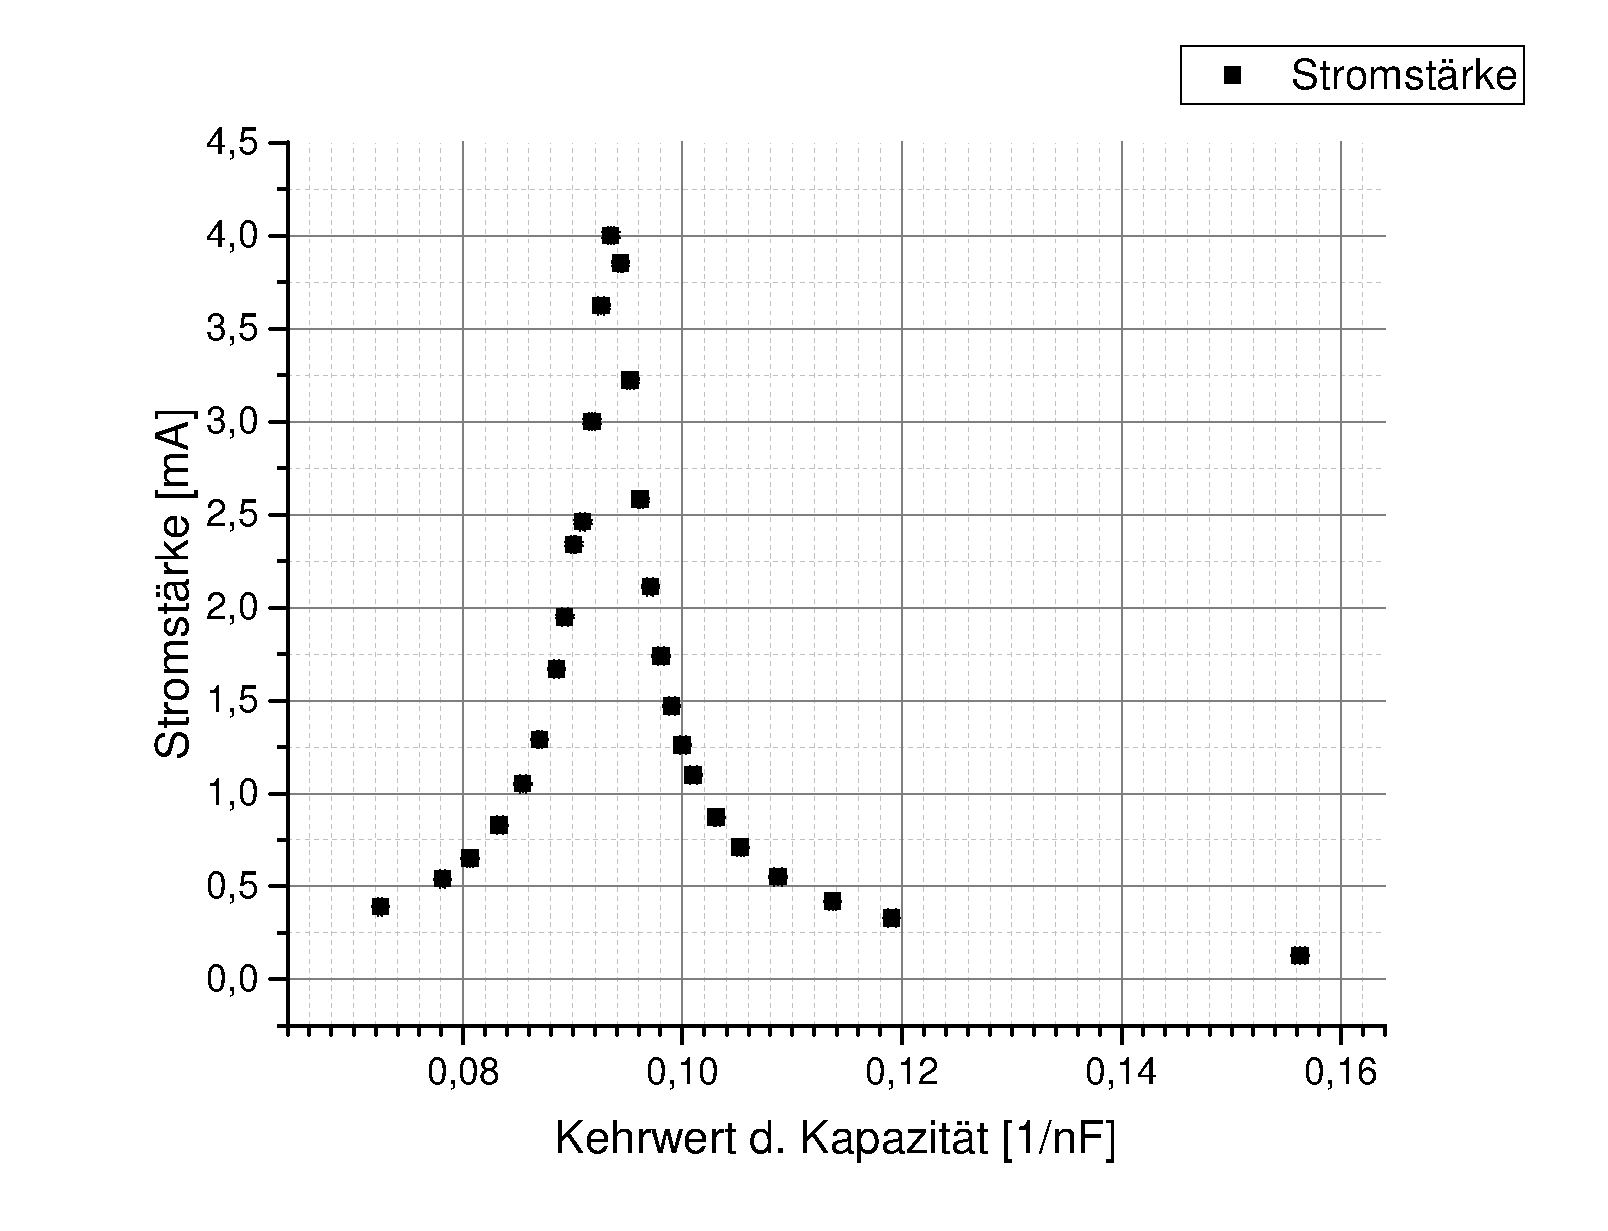
\includegraphics[width=0.7\textwidth]{Serie_0}
		\centering
		\caption{Hier ist die Stromstärke $ \left| I \right| $ gegen den Kehrwert der Kapazität bei $ R_v = \SI{0}{\ohm} $ aufgetragen. Die Fehlerbalken sind kleiner als die Symbolgröße.}
		\label{Serie_0}
		\centering
	\end{figure} 
	\begin{figure}[H]
		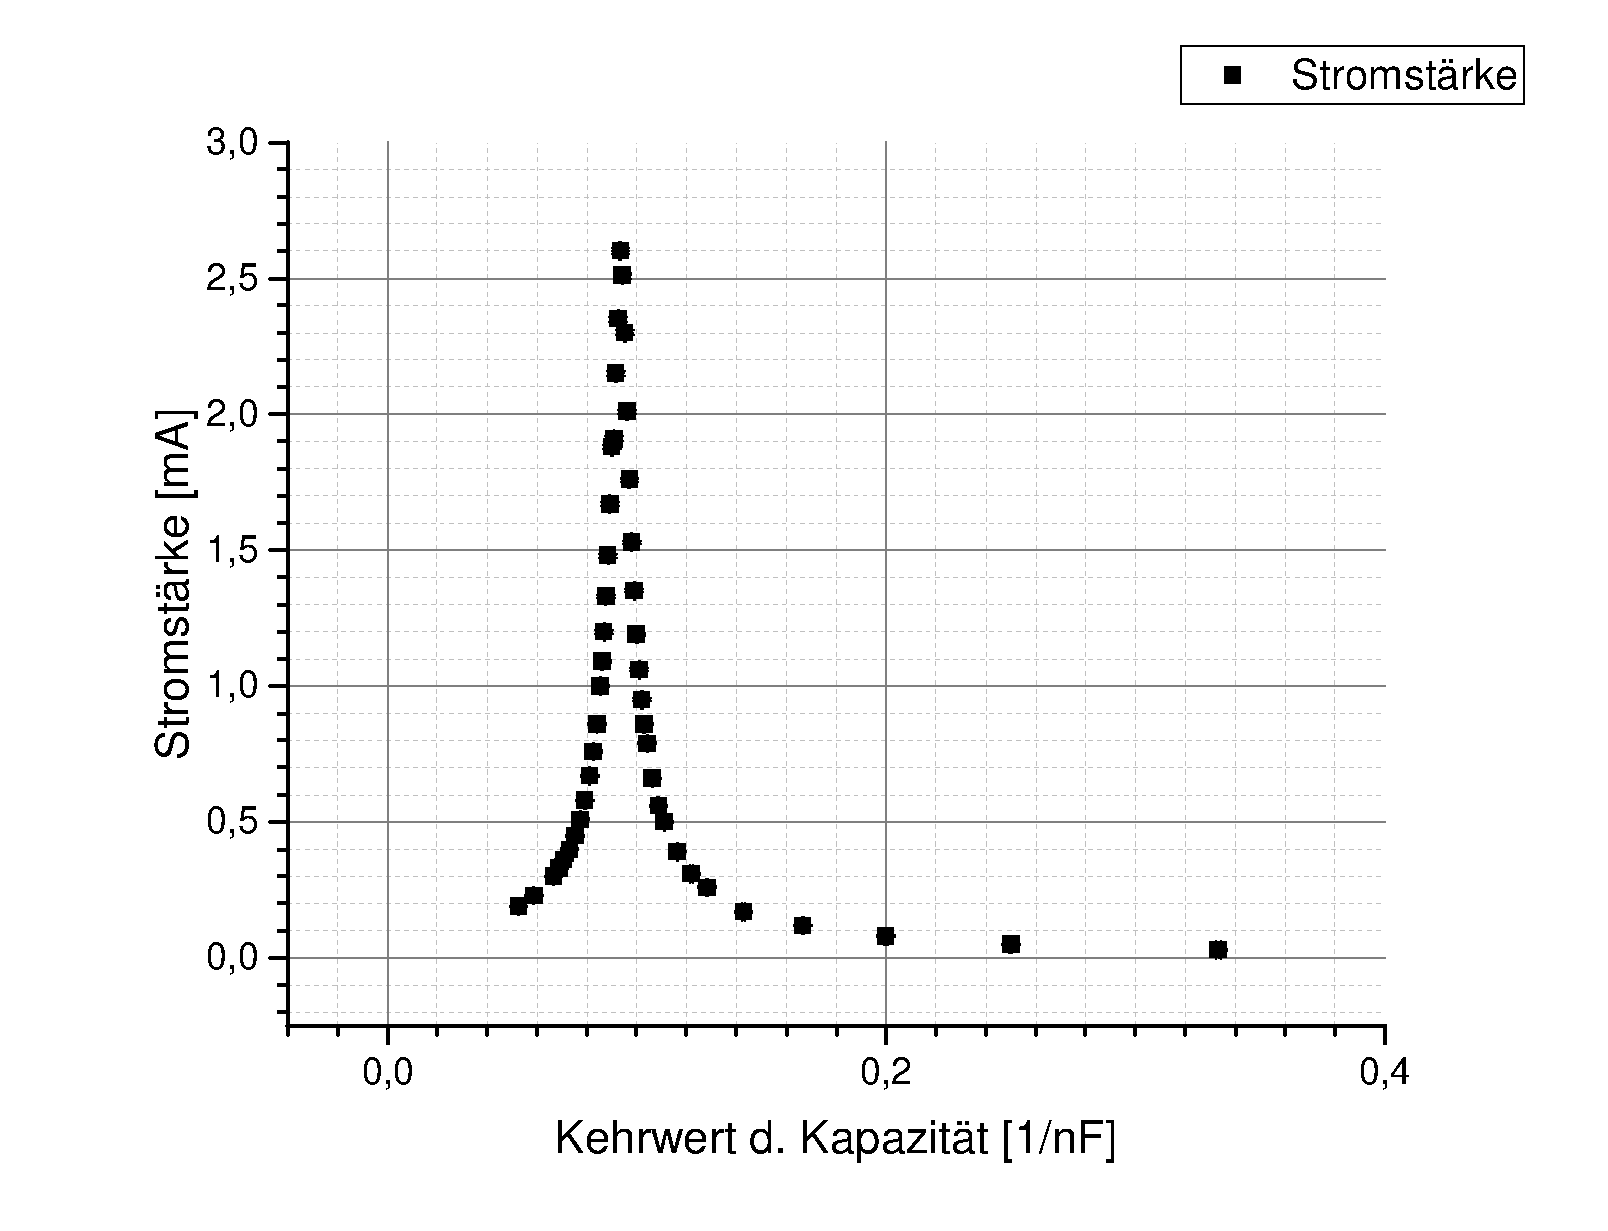
\includegraphics[width=0.7\textwidth]{Serie_200}
		\centering
		\caption{Hier ist die Stromstärke $ \left| I \right| $ gegen den Kehrwert der Kapazität bei $ R_v = \SI{200}{\ohm} $  aufgetragen. Die Fehlerbalken sind kleiner als die Symbolgröße.}
		\label{Serie_200}
		\centering
	\end{figure} 
	\begin{figure}[H]
		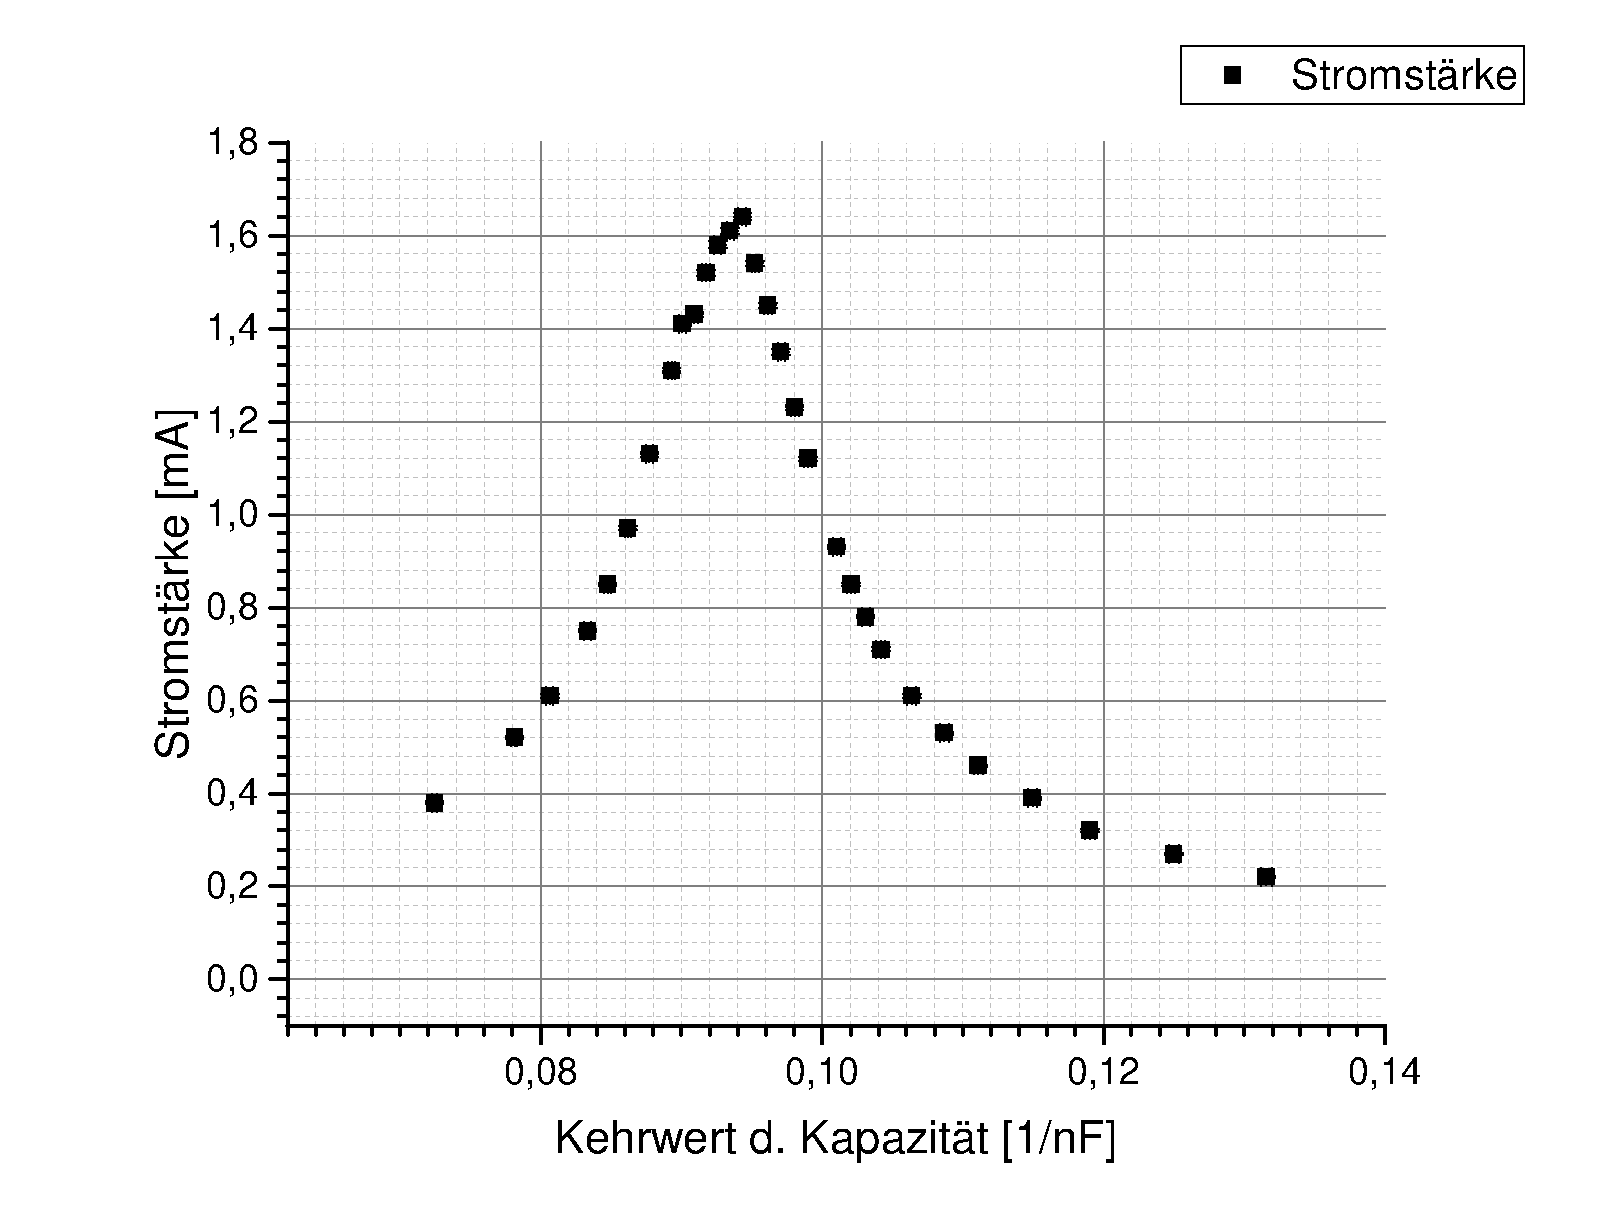
\includegraphics[width=0.7\textwidth]{Serie_500}
		\centering
		\caption{Hier ist die Stromstärke $ \left| I \right| $ gegen den Kehrwert der Kapazität bei $ R_v = \SI{500}{\ohm} $ aufgetragen. Die Fehlerbalken sind kleiner als die Symbolgröße.}
		\label{Serie_500}
		\centering
	\end{figure} 
	Es gilt nach der Thomsonschen Schwingungsformel:
	\begin{equation}
		\omega_0^2=\frac{1}{LC}
	\end{equation}
	Daraus ergibt sich im Fall der Variation von $C$ und festem $\omega$ am Maximum $ C_\text{max} $:
	\begin{equation}
		L=\frac{1}{\omega^2 C_0}
		\label{Thomson}
	\end{equation}
	
	Für den Verlustwiderstand $R$ gilt für die Orte $C_i$ an denen der Strom das $ 1/\sqrt{2} $-fache des Maximums annimmt:
	\begin{equation}
		R= \frac{2}{2\omega_0 \left( \frac{1}{C_2} - \frac{1}{C_1} \right)}
	\end{equation}
	Diese Orte wurden anhand der Diagramme abgelesen, was hierbei einen recht hohen Ablesefehler nach sich zieht.
	Für Verlustwiderstand und Induktivität ergibt sich die Unsicherheit gemäß \cref{Partielle_Unsicherheiten}.
	In \cref{Serie_Erg} sind die Ergebnisse aus Ablesen der Maxima und die daraus folgenden Induktivitäten der Spule sowie die Verlustwiderstände für die drei Messungen dargestellt.
	
	\begin{table}[H]
		\centering
		\begin{tabular}{ r | c | c | c }
			&\SI{0}{\ohm} & \SI{200}{\ohm} & \SI{500}{\ohm} \\ \hline
			$\left| I \right|_\text{max}$ /\si{mA} & $4\pm 0,03$ &$2,52\pm0,02$ & $1,64\pm 0,02$\\ 
			$1/C_\text{max}$ /\si{\per \nano \farad}& $0,095 \pm 0,004$ & $0,092\pm0,004 $&$0,0942\pm0,003$ \\
			$L$ /\si{\henry} & $2,41 \pm 0,1$ & $2,33\pm 0,1 $&$2,39\pm0,08$ \\
			$R$ /\si{\ohm}  &$ 398\pm 225$&$ 637\pm 225 $ & $796 \pm 225$\\
			$R_i$ /\si{\ohm} &$ 398\pm225$ & $437\pm225$ &$300,6\pm225$ \\
		\end{tabular}
		\caption{Abgelesene Maxima der Resonanzkurven und daraus berechnete Induktivitäten $L$ der Spule sowie Verlustwiderstände $R$ des Serienresonanzkreises bei den drei Messungen. Als Unsicherheit wurde hier eine nach oben abgeschätzte Ableseungenauigkeit (dreieckige WDF) gewählt. Diese ist sehr groß, da zwischen Messwerten interpoliert werden musste. Es ist deutlich erkennbar, dass die Unsicherheiten der Messpunkte demgegenüber verschwinden. Der Innenwiderstand wurde nach \cref{Verlust} berechnet.}
		\label{Serie_Erg} 
	\end{table}
	
	Im Serienresonanzkreis sollte für den Innenwiderstand der Spule gelten:
	\begin{equation}
		R_i=R-R_v
		\label{Verlust}
	\end{equation}
	Wenn man für die drei gewählten $R_v$ den Innenwiderstand der Spule auf diese Art und Weise ermittelt, erhält man die Ergebnisse, die in \cref{Serie_Erg} als $R_i$ dargestellt sind mit den Unsicherheiten gemäß \cref{Partielle_Unsicherheiten}.
	Hierfür wurde der Innenwiderstand der Spule, der durch Gleichstrommessung ermittelt wurde, benutzt.
	\subsubsection{Parallelresonanzkreis}
	
	In \crefrange{Para_2k}{Para_inf} ist die Stromstärke im Serienresonanzkreis gegen die Kapazität bei unterschiedlichen Widerständen $ R_v $ aufgetragen.
	\begin{figure}[H]
		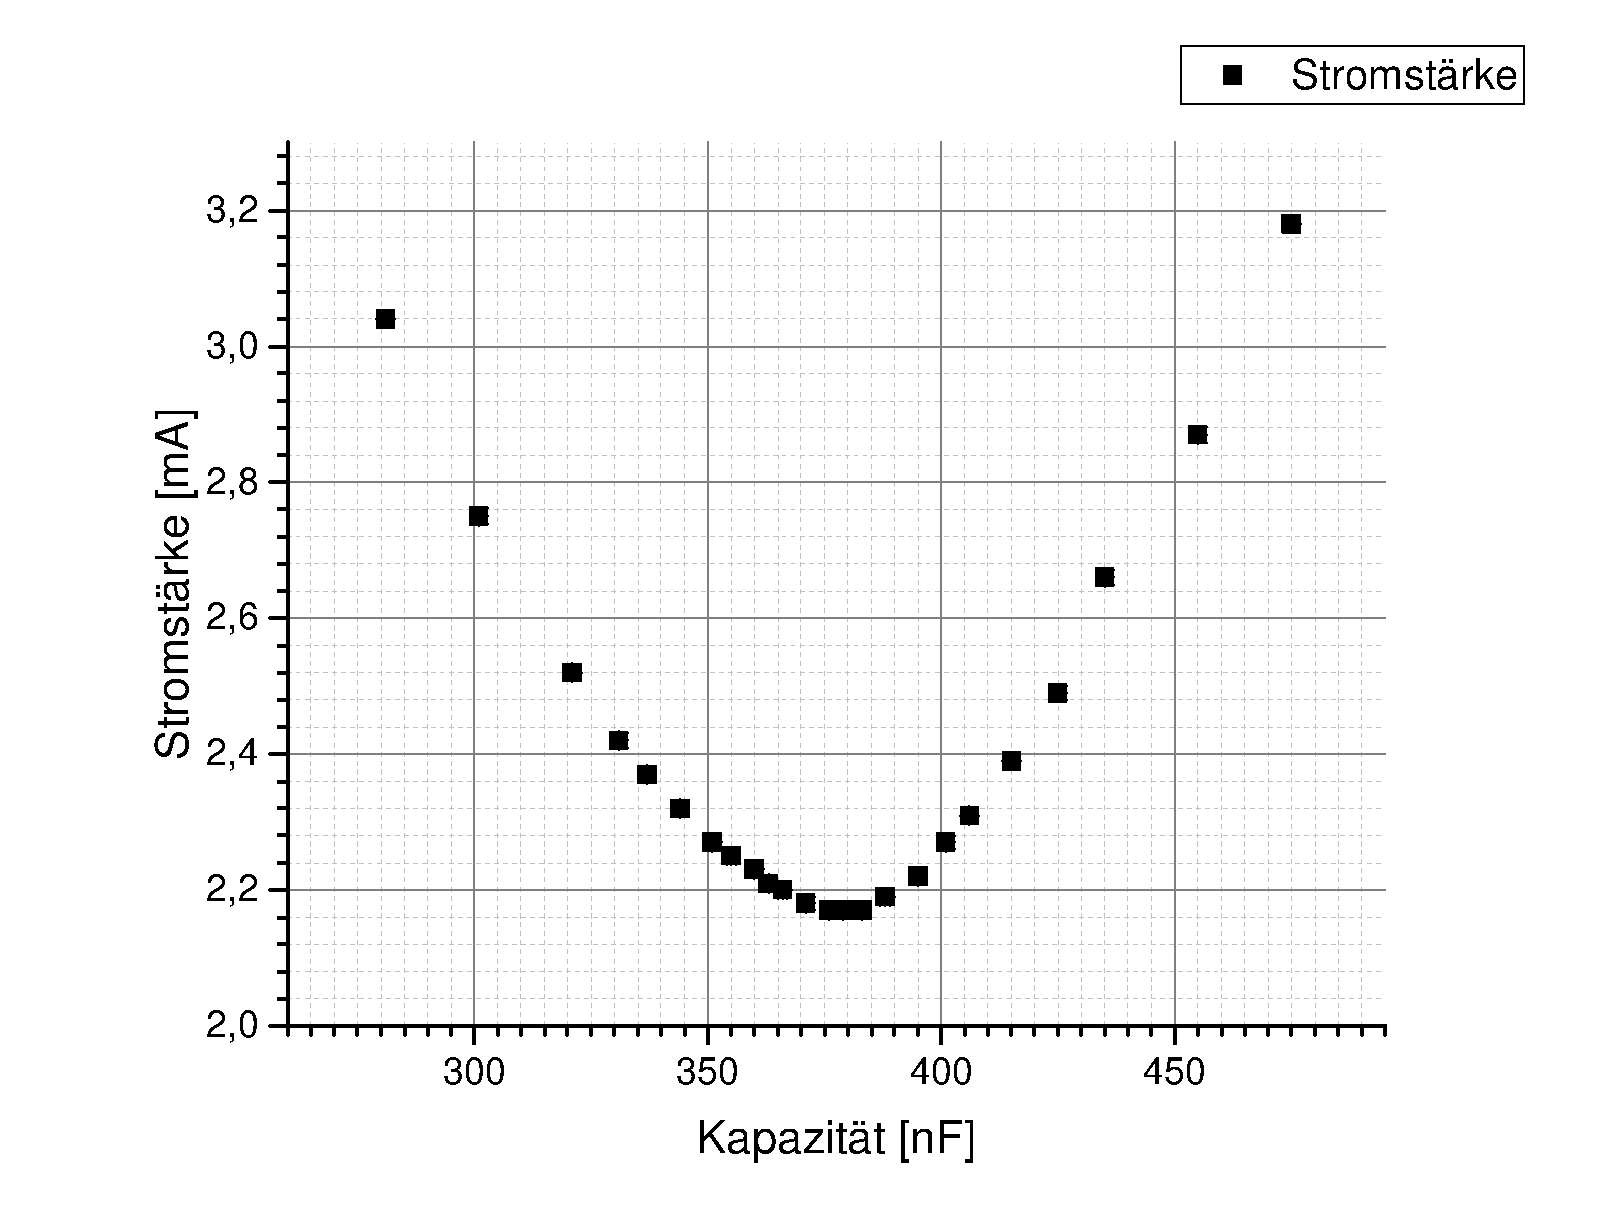
\includegraphics[width=0.7\textwidth]{Parallelstromkreis_2k}
		\centering
		\caption{Hier ist die Stromstärke $ \left| I \right| $ gegen die Kapazität bei $ R_p = \SI{2}{\kilo \ohm} $ aufgetragen. Die Fehlerbalken sind kleiner als die Symbolgröße.}
		\label{Para_2k}
		\centering
	\end{figure} 
	\begin{figure}[H]
		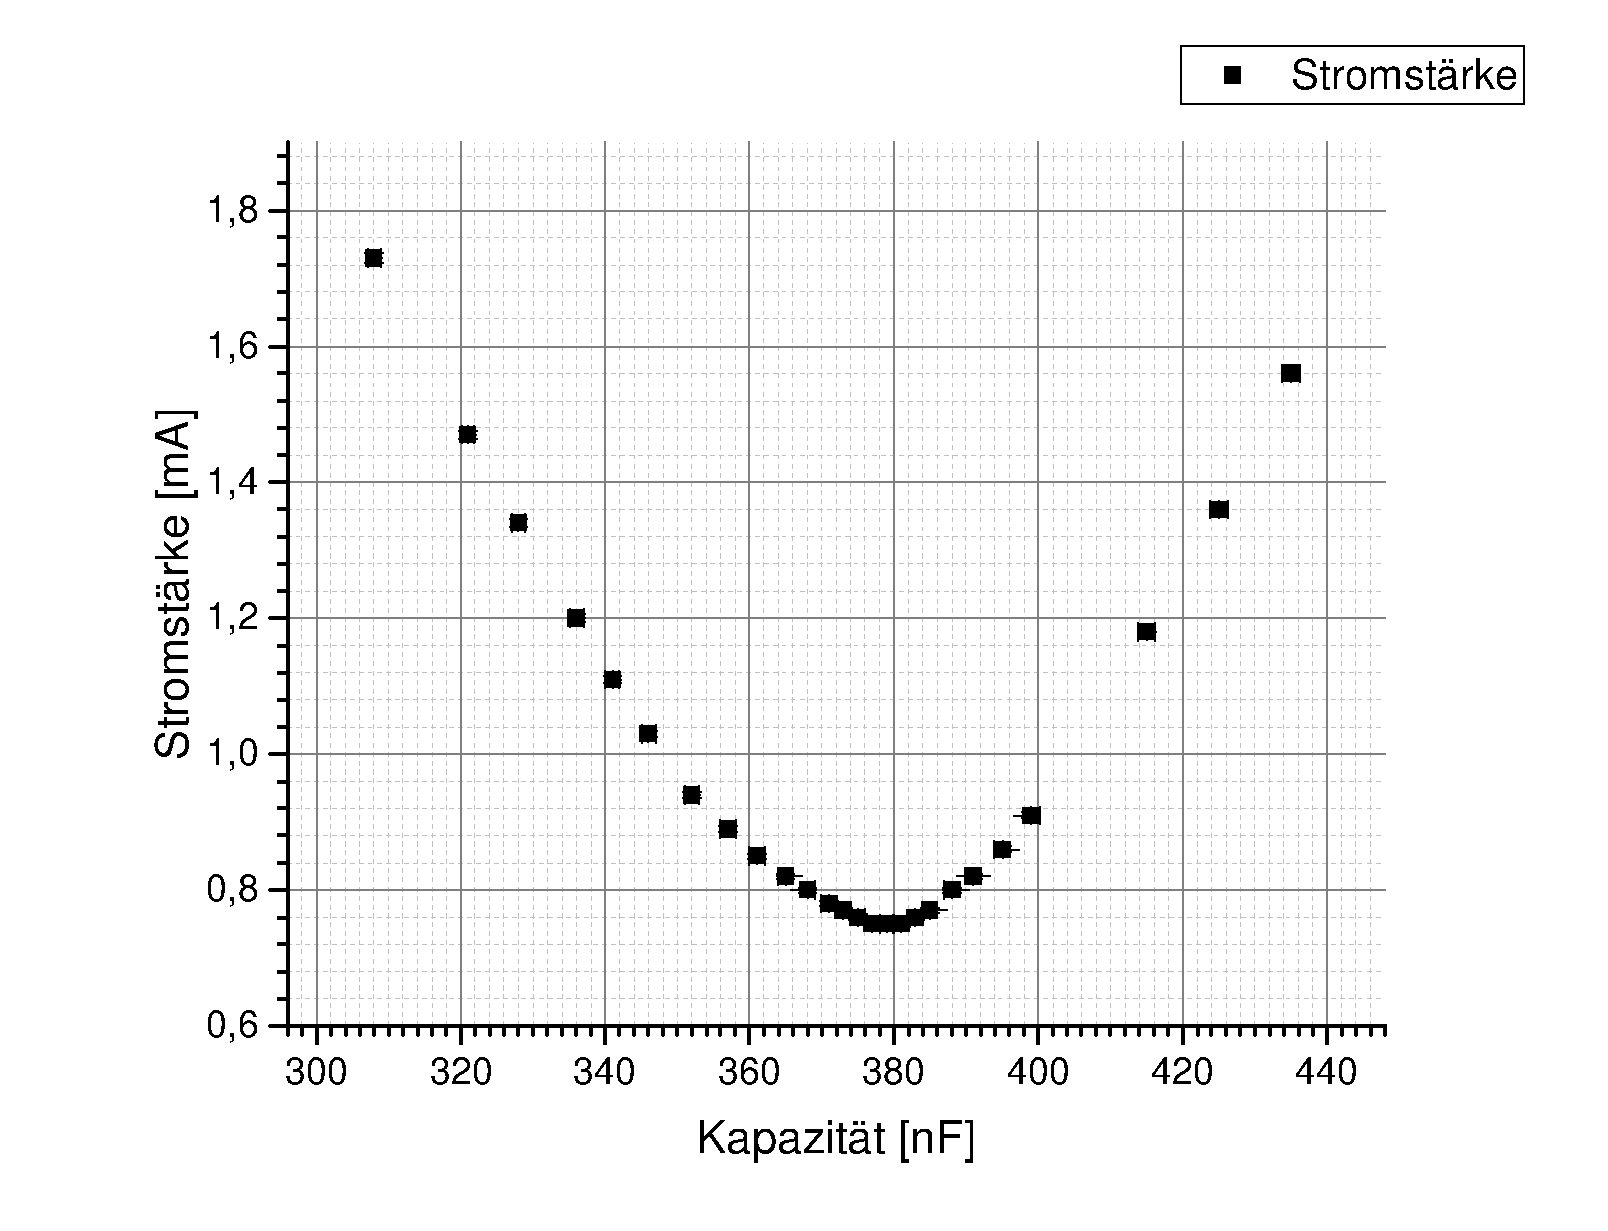
\includegraphics[width=0.7\textwidth]{Parallelstromkreis_10k}
		\centering
		\caption{Hier ist die Stromstärke $ \left| I \right| $ gegen die Kapazität bei $ R_p = \SI{2}{\kilo \ohm} $ aufgetragen. Die Fehlerbalken sind kleiner als die Symbolgröße.}
		\label{Para_10k}
		\centering
	\end{figure} 
	\begin{figure}[H]
		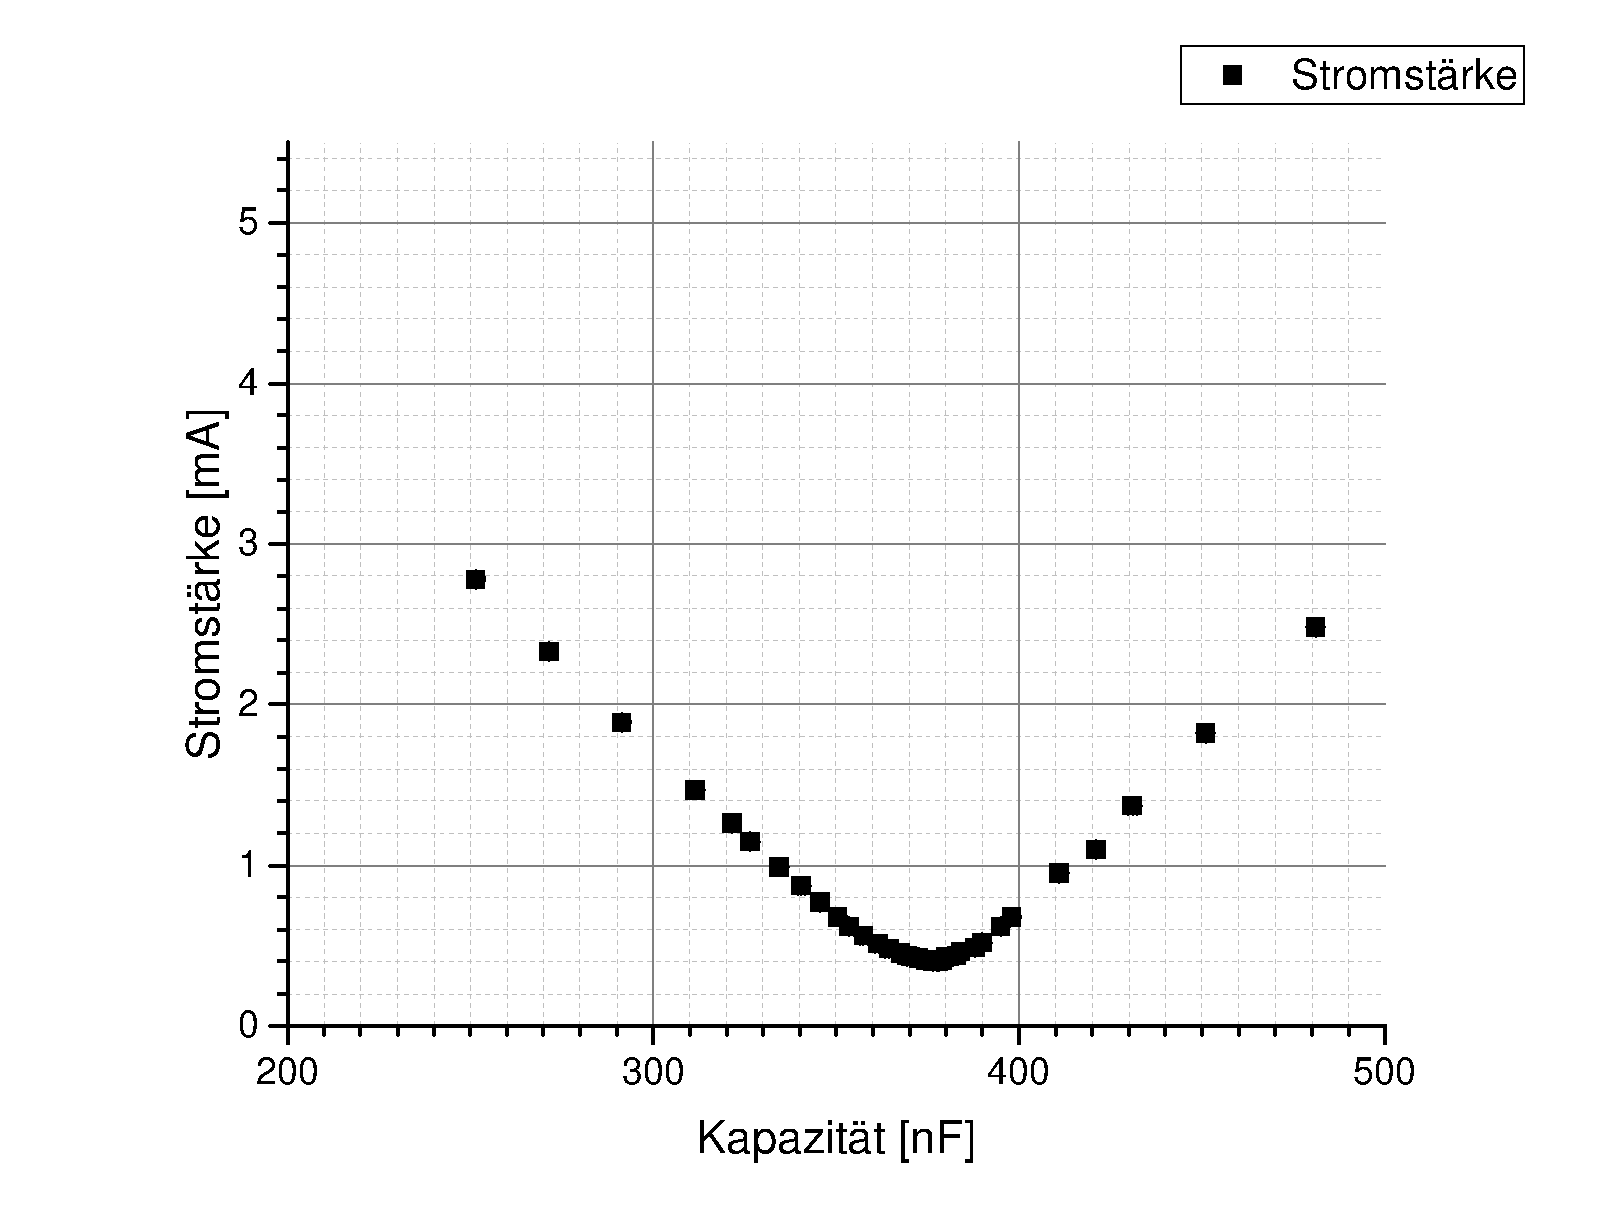
\includegraphics[width=0.7\textwidth]{Parallelstromkreis_inf}
		\centering
		\caption{Hier ist die Stromstärke $ \left| I \right| $ gegen die Kapazität bei unendlich großem Widerstand aufgetragen. Die Fehlerbalken sind kleiner als die Symbolgröße.}
		\label{Para_inf}
		\centering
	\end{figure}
	
	In \cref{Para_Erg} sind die Ergebnisse aus Ablesen der Maxima und die daraus folgenden Induktivitäten der Spule sowie die Verlustwiderstände für die drei Messungen dargestellt.
	Auch hier gilt \cref{Thomson}.
	Für den Verlustwiderstand $R$ gilt für die Orte $C_i$ an denen der Strom das $ \sqrt{2} $-fache des Minimums annimmt:
	\begin{equation}
	R= \frac{2}{2\omega_0 \left( C_2 - C_1 \right)}
	\end{equation}
	
	\begin{table}[H]
		\centering
		\begin{tabular}{ r | c | c | c }
			&\SI{2}{\kilo \ohm} & \SI{10}{\kilo \ohm} & inf  \\ \hline
			$  \left| I \right|_\text{min}$/\si{mA} & $2,17\pm 0,01$ &$0,75\pm 0,01$ & $0,041\pm 0,02$\\ 
			$C_\text{min}$ /\si{nF} &$380\pm2$&$379\pm2$&$376\pm2$\\
			$L$/\si{\henry} & $0,0666\pm 0,00035$ & $0,0668 \pm 0,00035$ & $0,0674\pm 0,00036$\\
			$R$/\si{\ohm} & $1675\pm 27$&$5584\pm 294$ & $9362\pm 826$\\
			$R_g$ /\si{\ohm} &$ 52,32\pm0,15$ & $252,3\pm0,600$ &$549,7\pm1,45$ \\ %TODO
		\end{tabular}
		\caption{Abgelesene Minima der Resonanzkurven und daraus berechnete Induktivitäten $L$ der Spule sowie Verlustwiderstände $R$ des Parallelresonanzkreises bei den drei Messungen. Als Unsicherheit wurde hier eine nach oben abgeschätzte Ableseungenauigkeit (dreieckige WDF) gewählt. Es ist deutlich erkennbar, dass die Unsicherheiten der Messpunkte selbst demgegenüber verschwinden.}
		\label{Para_Erg} 
	\end{table}
	\subsection{Diskussion}
	Eine Änderung des Widerstandes im Resonanzkreis führte zu keiner anderen Eigenfrequenzen und stimmt mit der Theorie $\omega_0 = \frac{1}{\sqrt{LC}}$ überein. %TODO cref auf Tabelle mit Werten
	Auf den Spulen waren keine Induktivitäten angegeben, insofern ist es nicht möglich unsere bestimmmten Werte mit Werten des Herstellers zu verleichen.
	Für die dicke Spule ergab sich eine gemittelte Induktivität von \SI{0,094 \pm 0,002}{H} (\cref{Serie_Erg}) und für die kleine Spule \SI{0,0669 \pm 0,0003}{H} (\cref{Para_Erg}).
	Die Unsicherheitsintervalle der Innenwiderstände, die einerseits durch das Multimeter und andererseits durch das Resonanzverhalten bestimmt worden sind überschneiden sich. 
	Folglich ist die Hypothese, dass sich mit dem Experiment der Innenwiderstand einer Spule erfasst werden kann, bestätigt.
	%TODO Bezug/Nutzten oder sonst was
	%TODO auch hier die Hypothese wiederholen
	
	\section{Schlussfolgerung}
	%TODO Rückgriff auf Hypothese und drittes Nennen dieser
	Die Hypothese wurde bestätigt, da die Fehler beider Messungen des Widerstands sich überschnitten.
	Auf dem einstellbaren Kondensator war keine Unsicherheit angegeben, daher mussten wir diese abschätzen.
	Außerdem war auf den Spulen keine Induktivität angegeben, daher konnte die durch die Eigenfrequenz bestimmte Induktivität nicht mit einem vorgegebenen Wert, bzw. des Unsicherheitsinterval, verglichen werden.
	Die Bestimmung des Innenwiderstand durch das Multimeter ist sehr viel praktikabler als durch eine Untersuchung der Resonanzkurve einese Resonanzschwingkreises untervariation der Kapazitäten.
	Von beiden Resonanzkreisen erwies sich der Parallelresonanzkreis als genauer zum Ermitteln der Induktivität der Spulen, da die relative Unsicherheit in Serie 2\% und parallel dagegen nur 0,4\% betragen hat.
	
	
	%TODO Quellen zitieren, Websiten mit Zugriffsdatum
	%TODO Verweise auf das Laborbuch (sind erlaubt)
	%TODO Tabelle + Bilder mit Beschriftung
	\printbibliography
\end{document}
